\documentclass{article}
\usepackage[utf8]{inputenc}
\usepackage{framed}
\usepackage{amsmath,amsthm,amsfonts,amssymb,amscd}
\usepackage[a4paper,hmargin=0.8in,bottom=1.3in]{geometry}
\usepackage{lastpage,enumerate,fancyhdr,mathrsfs,xcolor,graphicx,listings,hyperref,enumitem}
\author{Hardik Rajpal}
\title{Notes from John C. Hull's famed textbook.}
\hbadness 100001
\begin{document}
\maketitle
\section{Chapter 1: Introduction}
A \textbf{derivative} can be defined as a financial instrument whose value depends on (or
derives from) the values of other, more basic, underlying variables. The variables 
underlying a derivative are often the prices of traded assets. A stock option is a
derivative whose price is dependent on the price of the stock. Note that derivatives
can be dependant on almost any variable: from the price of hogs to the amount
of snow in the Alpes.
\subsection{Exchange-Traded Markets}
A derivatives exchange is a market where individuals trade standardized contracts that
have been defined by the exchange. Traditionally, derivative exchanges used the 
\emph{open outcry system}; physically meeting up on the floor of the exchange, shouting
and using a set of complicated hand signals. This is fortunately being replaced by
electronic trading. The replacement has led to a growth in algorithmic trading,
also known as blackbox trading, automated trading, high-frequency trading, or robo trading,
or beep-boop-machine-make-money-out-of-thin-air trading. The last one is rarely used in
the industry.
\subsection{Over-the-counter Markets}
This is an alternative to the exchange market and has become \textbf{much larger} than it in terms
of the total volume of trading. Trades are done over the phone and usually between
two fininsts or between a fininst and one of its clients (typically a corporate treasurer
or a fund manager). Fininsts often act as \textbf{market makers} for the more commonly
traded instruments; they are prepared to quote a bid price (to buy) and offer price (to sell).
There is a credit risk associated with over-the-counter trade, while exchanges have
organized themselves to eliminate virtually all credit risk.
\subsection{Forward Contracts}
A type of derivative that is an agreement to buy or sell an asset at a certain
future time for a certain price (is a \textbf{forward contract}). In contrast,
a \textbf{spot contract} is an agreement to buy or sell an asset today. These
appear in over-the-counter trades. Each party
involved in a forward contract can assume one of two positions:
\begin{enumerate}
    \item the \textbf{long} position: agreeing to \textbf{buy} the asset at the specified date and price.
    \item the \textbf{short} position: agreeing to \textbf{sell} the asset at the specified date and price.
\end{enumerate}
The payoff from a \textbf{long} position in a forward contract on one unit of an asset is: $S_T - K$, where
$K$ is the delivery price (the one agreed to by both parties) and $S_T$ is the spot price of the asset
at maturity of the contract. The payoff in the \textbf{short} position is negative of that in the long
position: $K-S_T$. As forward contracts cost nothing to enter, these payoffs are also the net gain or loss
associated with the contract.\\
Forward contracts can be used in the landscape of stocks to benefit from expected changes in stock prices:
\begin{itemize}
    \item If a stock is expected to drop ($\implies$ have a lower $S_T$ in the near future), enter a forward
    contract to buy the stock in the future at $K<\text{current price}$, having sold it now at the current price.
    \item If a stock is expected to rise ($implies$ have a higher $S_T$ in the near future), enter a forward
    contract to sell the stock in the future at $K>\text{current price}$, having sold it now at the current price.
\end{itemize}
Both these points assume enough profit is made to justify any loans involved.
\subsection{Futures Contracts}
They are also agreements to buy/sell an asset at a certain time at a certain price, but are traded on an exchange.
The commodities include pork bellies, live cattle, sugar, wool, lumber,
copper, aluminum, gold, and tin. The financial assets include stock indices, currencies,
and Treasury bonds. Future prices are regularly reported in the financial press.
\subsection{Options}
Options are traded both on exchanges and in the over-the-counter market. There are two types:
\begin{enumerate}
    \item Call option: Gives the holder the right to buy the underlying asset by a certain date for a certain price.
    \item Put option: Gives the holder the right to sell the underlying asset by a certain date for a certain price.
\end{enumerate}
The specified price is called the \textbf{exercise price or strike price}, while
the specified date is called the \textbf{expiration date or maturity}. Note that 
\textbf{American} options can be exercised at any date on or before the expiration, while
\textbf{European} options can only be exercised on the expiration date.\\
The option gives the holder the right to exercise a trade; they don't have to actually make
the trade. This freedom comes at a cost; precisely, the cost to acquiring an option.
\subsubsection{Properties of Options}
\begin{itemize}
    \item The price of a call option decreases as the strike price increases,
    while the price of a put option increases as the
    strike price increases. (Is this because the prices is in general expected to drop,
    and hence buying at a higher price (call option with high strike price)
    is less preferred while selling at a higher price (put option with higher strike price)
    is more preferred?).
    \item However, both types of options become more valuable as 
    their time to maturity increases.
\end{itemize}
Consider a case where an investor buys a call option with the asset as 100 shares of Google,
the strike price as \$520 per share and the expiration date as 18/12/10, at a price of \$32 per share.
\begin{itemize}
    \item The investor has spent \$3200 in acquiring the option.
    \item If Google's share price doesn't rise above \$520 by the expiration date,
    the investor has no reason to exercise the option (paying \$520 for a share while the
    bid price is much below that) and has thus lost \$3200.
    \item If before the expiration date, Google's share price rises above \$520, the investor can
    exercise the option; buy the shares at \$520, and sell them at the current price $S_T$, making
    a profit of $100(S_T-(520+32))$.
    \item Note that we're neglecting TVoM here.  
\end{itemize}
The person who sells the put option is obliged to do the buying at the option's maturity (or before).
Consider a case where an investor sells a put option with on 100 shares of Google with the 
strike price as \$480 per share and the expiration date as 18/09/10, at a price of \$22.2 per share.
\begin{itemize}
    \item Immediately, the investor receives a cash inflow of $100\times22.2=\$2220$
    \item Suppose Google's share price up to the expiration date remains above \$480, the buyer of the
    option has no incentive to sell his shares at \$480, and doesn't exercise the option.
    \item Suppose Google's share price $S_T$ is below \$480 before the expiration date, the buyer of the option
    sells the shares back to the investor at \$480, and buys them at $S_T$ making a profit of: $100\times(480-(S_T+22.2))$.
    \item In this case, the investor is forced to buy shares worth $S_T<480$ at 480, and suffers a net loss of:
    $100\times(480-(S_T+22.2))$.
    \item The investor's gain can be defined as 100 times $S_T+22.2 - 480$ when $S_T < 480$ and as 22.2 when $S_T>480$.
\end{itemize}
The diagrams below summarize the two analyses with the assumption
of European options.
\begin{center}
    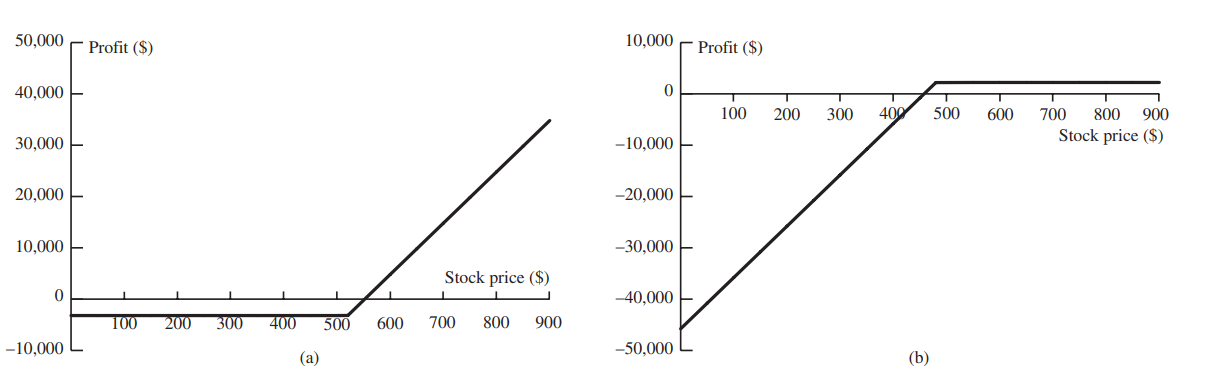
\includegraphics[width=6in]{rsrc/trading-options.png}
\end{center}
Note that there are four types of participants in the options market with
the choice of put/call option and buying or selling the option. Buyers are said
to take \textbf{long positions} and sellers are said to take \textbf{short positions}.
Selling an option is also known as \textbf{writing an option}.
\subsection{Types of Traders}
Derivatives markets have been successful mainly because of the variety of traders
they have attracted and their great deal of liquidity. When an investor wants to take
one side of a contract, there is usually no problem in finding someone who is prepared
to take the other side. Traders can be broadly divided into three categories:
\begin{enumerate}
    \item Hedgers: use derivatives to reduce the risk they face from potential future movements
    in a market variable.
    \item Speculators: use derivatives to bet on the future direction of a market variable.
    \item Arbitrageurs: take offsetting positions in two or more instruments to lock in a profit. 
\end{enumerate}
\subsection{Hedgers}
Hedgers can use future contracts to, for example, hedge the risk of foreign exchange. Companies
that agree to pay a fixed amount in a currency, say C2, different from their operating currency,
say C1, can buy futures of the amount in C2 at a fixed price in C1; hence avoiding any loss
due to fluctuations in the exchange rate between C1 and C2. Conversely, a company set to receive
a payment in C2 in the future can sell futures of C1 at the current exchange rate to hedge
the foreign exchange risk. It should be noted that the companies may have been better off
without using the future contracts, but they could have been worse off too.\\
``The purpose of hedging is to reduce risk. There is no guarantee that the outcome with
hedging will be better than the one without hedging.''\\
\subsubsection{Hedging with Options}
We use options to hedge against the possible decline in the price of shares held by us. One method
is to buy put options at a high enough strike price $K$ to lower-bound our possible loss by $CP-K$,
where $CP$ is the current price of the shares.
\begin{itemize}
    \item If the price drops below K, we exercise our option
    to sell the shares at $\$K$ and buy them back at the lower price.
    \item If the price doesn't drop below K, we don't exercise our option, we have lost the amount
    we paid for the option, but we've been protected from the risk.
\end{itemize}
We note that options provide a lower bound for the loss incurred by price dips, while retaining
the possibilty to earn from price rises. Futures, however, fix the price to protect against
price dips but also keep us from benefitting from price rises.
\subsection{Speculators}
Speculators are either betting on the price of an asset going down or going up.
\subsubsection{With Futures}
Suppose a speculator believes that C2 will be increasingly more valuable than C1
over the next few months. The speculator can:
\begin{itemize}
    \item Purchase, say 250,000 of C2 right away and sell it when it becomes more valuable.
    \item Enter the long position on a future implying the purchase of 250,000 of C2 at a rate $K$
    lower than the expected exchange rate in the future. Then, on the expiration date, we 
    purchase 250,000 of C2 at this lowered rate and immediately sell it for a profit given by:
    $250,000\times(S_T-K)$
\end{itemize}
Note that if the futures's promised price is lower than the current exchange rate, the profit obtained
is even larger than that obtained by the first option, while the loss is reduced in magnitude too.
The futures market allows the speculator to take a large speculative position with a relatively
small initial outlay. 
\subsubsection{With Options}
Options allow for more profit (and equivalently, more loss, albeit capped at
the capital) to be made with the same investment capital,
than would be made by purchasing shares rightaway. This is because options themselves are much cheaper
than shares. The only reason the profit/loss is magnified is because you can buy more options with the
same capital right now than you can buy shares. Summary: Good outcomes are magnified, while with
bad outcomes, the entire initial investment is lost.
\subsubsection{Comparison}
It's important to note that with futures, both the loss and gain are unbounded but with options, the 
loss is bounded below by the amount paid for the options.
\subsection{Arbitrageurs}
Arbitrage involves locking in a riskless profit by simultaneously entering into transactions in two or
more markets. A simple example of arbitrage involves selling and buying stocks listed in different
markets in different currencies and profiting from the lag from the exchange rate. Small investors
are left with neglegible profits in this scheme in light of transaction costs, but large investors
make significant profits. Arbitrage opportunities don't last very long and such lags are temporary
and fleeting.
\subsection{Dangers}
Sometimes, traders who have a mandate to be hedgers or arbitrageurs, become (by
choice or ignorance) speculators; this can lead to disastrous effects. Risk management
is an important part of trading firms and should be carried out without any negligence.
\section{Chapter 2: Mechanics of Futures Markets}
The (current) price of future contracts of a particular asset are determined by the laws of demand and supply:
\begin{itemize}
    \item more buyers $\implies$ price goes up $\implies$ more sellers enter the market.
    \item more sellers $\implies$ price goes down $\implies$ more buyers enter the market.
\end{itemize}
\subsubsection*{Closing Out Positions}
Most futures contracts do not lead to delivery because most traders choose to close out their positions
prior to the delivery period specified in the contract. Closing out refers to entering into futures
contracts that exactly counter your current long or short position on an asset, by having \textbf{the same amount
of the asset in the opposite position} with \textbf{the same delivery period}. The loss/gain arises
from the fact that the countering future is purchased at a much later date (which is probably close
to the delivery period) and hence the price specified in the future is different from those entered previously.
The loss/gain is determined by the change in the futures price between the first contract and the counter contract.
We still review the delivery arrangements in futures contracts  because the possibility of a final delivery
ties the futures price to the spot price.
\subsection{Specs of a Futures Contract}
The futures contract must specify:
\begin{itemize}
    \item The asset
    \item The contract size (how much of the asset is being traded)
    \item Where the delivery will be made
    \item When the delivery will be made
\end{itemize}
Additionally, some alternatives are specified for the grade of the asset that will be delivered
or for the delivery locations. When the party with the short position is ready to deliver,
it files a \emph{notice to deliver} with the exchange, specifying the selections it has made
with respect to said alternatives.
\subsubsection*{The Asset}
Exchanges (the institutes organizing trades) put down the criterion for acceptable grades
and respective prices of assets that are commodities. For ex., corn bushels can be described
as as No.1 Yellow, No. 2 Yellow and No. 3 Yellow; each with no further than 1.5 cents from its
centre color category. The financial assets in futures contracts are generally well-defined. For ex.
the Japanese Yen. Treasury bonds and notes on the CBoT have some interesting features here.
\footnote{The underlying asset in the Treasury bond
contract is any long-term US Treasury bond that has a maturity of greater than 15 years and
is not callable within 15 years. In the Treasury note futures contract, the underlying
asset is any long-term Treasury note with a maturity of no less than 6.5 years and no
more than 10 years from the date of delivery. In both cases, the exchange has a formula
for adjusting the price received according to the coupon and maturity date of the bond
delivered.} 
\subsubsection*{Contract Size}
It specifies the amount of the asset to be delivered under one contract. A very large size is unusable
by investors who wish to hedge relatively small exposures or take relatively small speculation positions while
a very small size may render the contract expensive to trade because of costs associated with each trade; contract
sizes are an important decision for the exchange. The correct size of a contract depends on the likely user, and 
exchanges have introduced minicontracts to attract small investors: mini-Nasdaq.
\subsubsection*{Delivery Arrangements}
The exchange must specify the delivery spot; it's particularly important for commodities with large transportaion
costs, like giant vipers. When alternative delivery locations are specified, the price received by the short position party
is adjusted base on the location chosen by the party: price tends to be higher for delivery locations that are
relatively far from the main sources of the commodity.
\subsubsection*{Delivery Months}
A futures contract is referred to by its delivery month, but the contract must specify the precise period of delivery.
Though for many futures contracts, the period is the entier month. The delivery months vary from contract to contract
and are chosen by the exchange to meet the needs of the market participants.
\begin{itemize}
    \item At any given time, contracts trade for the closest delivery month and a number of subsequent
    delivery months.
    \item The exchange specifies when trading in a particular month's contract
    will begin.
    \item The exchange also specifies the last day on which trading can take place for a
    given contract.
    \item Trading generally ceases a few days before the last day on which delivery
    can be made.
\end{itemize}
\subsubsection*{Prices, Positions and Limits}
The exchange further defines how prices will be quoted: the currency and precision.
The exhange also specifies daily price movement limits for most contracts. The contract
is said to be:
\begin{itemize}
    \item limit down if it has moved down by the limit from yesterday's closing price.
    \item limig up if it has moved up by the limit from yesterday's closing price.
\end{itemize}
A \emph{limit move} is a move in the either direction that crosses the limit. Normally, trading
ceases for the day when a contract is limit up or limit down, but, in some instances, the exchange
has the authority to step in and change the limits. The daily price limits prevent large movements
in price from occuring because of speculative excesses, but they can become a barrier to trading
when the price of an underlying commodity is in fact shifting rapidly; price limits remain controversial
in terms of their effect on the futures market. \textbf{Position limits} are the maximum number of contracts
that an speculator (any investor?) may hold. These limits prevent the speculators from exercising undue
influence on the market.
\subsection{Convergence of Future Price and Spot Price}
The futures price converges to the spot price of the underlying asset as the delivery period comes closer; at
the delivery period the future price is practically equal to the spot price. The reason for this is the 
opportunity for arbitrage while the prices are far apart:
\begin{itemize}
    \item If cost(futures)$>$cost(asset), traders will short futures contracts, delivering with the assets bought at a lower cost.
    \item If cost(futures)$<$cost(asset), companies interested in acquiring the asset will enter long positions in futures contracts
    instead of buying the asset, thus making the futures more valuable.
\end{itemize}
\subsection{The Operation of Margins}
One of the key roles of the exchange is to organize trading so that contract defaults are avoided.
\subsubsection*{Daily Settlements}
This refers to practice of adjusting the investor's \emph{margin account} at the end of a day to reflect the investor's 
loss or gain. The account also contains deposits known as \emph{initial margins}, which need to be deposited on entering
futures contracts. The investor's profit at the end of the day is given by:
\begin{equation}
    \sum_{i \in [n]}{(\text{spot price of asset i} - \text{strike price of futures contract of asset i in long position})}
\end{equation}
and negative terms for futures in short positions.
The margin account is altered by this amount at the end of each day. Hence, initial margins are determined by the asset's price
and the expected variation. Note that the previous days alteration is first undone, to avoid the incorrect accumulation
or gain/loss brought about by a constant difference between the future's strike price and the spot price. A trade is first
settled at the close of the day on which it takes place. It is then settled at the
close of trading on each subsequent day. Note that money actually moves from the investor's margin account to their broker,
and then to traders in the opposite position who are profiting in the other direction because of the gap between the future's
strike price and the spot price.\\
We also have the notion of a \textbf{maintenance margin}, whose role is to ensure the margin account's balance doesn't go into 
negative values. The investor is rung up when hte margin account's balance falls below this value and the investor is expected
to top up the balance to the initial margin level by the end of the next day. The extra funds provided in the margin account 
are known as \textbf{variation margin}; in the absence of a variation margin, the broker closes out the position.
\section{Investopedia Summaries}
\subsection{\href{https://www.investopedia.com/terms/c/cash-and-carry-arbitrage.asp}{Cash and Carry Arbitrage}}
It's a market neutral strategy combining:
\begin{itemize}
    \item purchase of a long position in an asset such as a stock or commodity
    \item sale (short) of a position in a futures contract on that same underlying asset.
\end{itemize}
The strategy seeks to exploit pricing inefficencies between spot and futures markets for an asset.
We ``carry'' the asset for physical delivery until the expiry date of the futures contract.
The strategy involves the risk of expenses associated with physically ``carrying'' an asset until expiry, but
the risk of market movement, the major component in any regular long or short trade is mitigated.
For profits, the futures contract must be theoretically priced above the stock.
\begin{center}
\begin{framed}
    Strategy is viable only if cash inflow from the short futures exceeds the acquisition costs
    and carrying costs on the long asset position.
\end{framed}
While arbitrage in non-physical assets, such as stock indices, requires only financing costs,
(as opposed to arbitrage in physical markets, which also requires storage and insurance of the 
associated commodities), the barrier to entry is also lower than that of arbitrage in physical
markets. Thus, more players enter the market and the spread between futures and spot prices
are very low, leading to fewer opportunities to profit.

\end{center}

\end{document}